\section{Systemarkitektur}
\label{chap:systemarkitektur}

Efter at have udarbejdet kravspecifikation, systemskitse og domain model, var der formet en idé om hvordan systemet skulle fungere. I det følgende beskrives hvordan systemarkitekturen er udformet. 

Systemarkitekturen er lavet ved brug af SysML og UML diagrammer. SysML bruges til beskrivelse af hardware, mens UML diagrammer bruges til beskrivelse af software. N + 1 og applikations modellen anvendes til udarbejdelse af UML diagrammer. Foruden SysML og UML diagrammer er der benyttet en række diagrammer, i det følgende beskrives overordnet nogle af de anvendte diagrammer.\\

\textbf{Use case}\\
Use cases og tilhørende diagrammer er benyttet i projektforløbets indledende faser. De bruges til at overskueliggøre systemets kunnen og opdele systemet i mindre dele. Use cases har i høj grad fungeret som et omdrejningspunkt, hvorfra stort set alt funktionalitet udspringer.

\textbf{Domainmodel}\\
Domain modellen er brugt som en overgang mellem kravspecifikation og systemarkitektur.
I kravspecifikation beskrives hvad der sker ved interaktion med systemet. Mens
systemarkitekturen bruges til at beskrive systemet i blokke og til at skitsere både interne
og eksterne forbindelser. Domain modellen bruges til at beskrive hele systemets domæne.
Der kigges ikke på hardware vs. software, der kigges i stedet på "enheder"og deres
ansvarsområder.

\textbf{SysML}\\
SysML diagrammer er benyttet til dokumentation af systemets hardware. Disse diagrammer er blevet anvendt til at tydeliggøre, hvilke hardware blokke der høre til hvor og hvordan de kommunikere.  

\textbf{UML}\\
UML diagrammer er benyttet til dokumentation af systemets software. Disse diagrammer anvendes til at forklare hvordan systemet er opbygget, hvordan de forskellige delsystemer snakker sammen og hvordan systemet funktionalitet generelt er opbygget.

\newpage
 
\subsection{Blokbeskrivelser}
Det overordnede bdd på figur \ref{fig:bdd_asd} viser hvilke hardware blokke systemet består af, samt hvilke parts blokkene indeholder.

\begin{figure}[H]
	\centering
	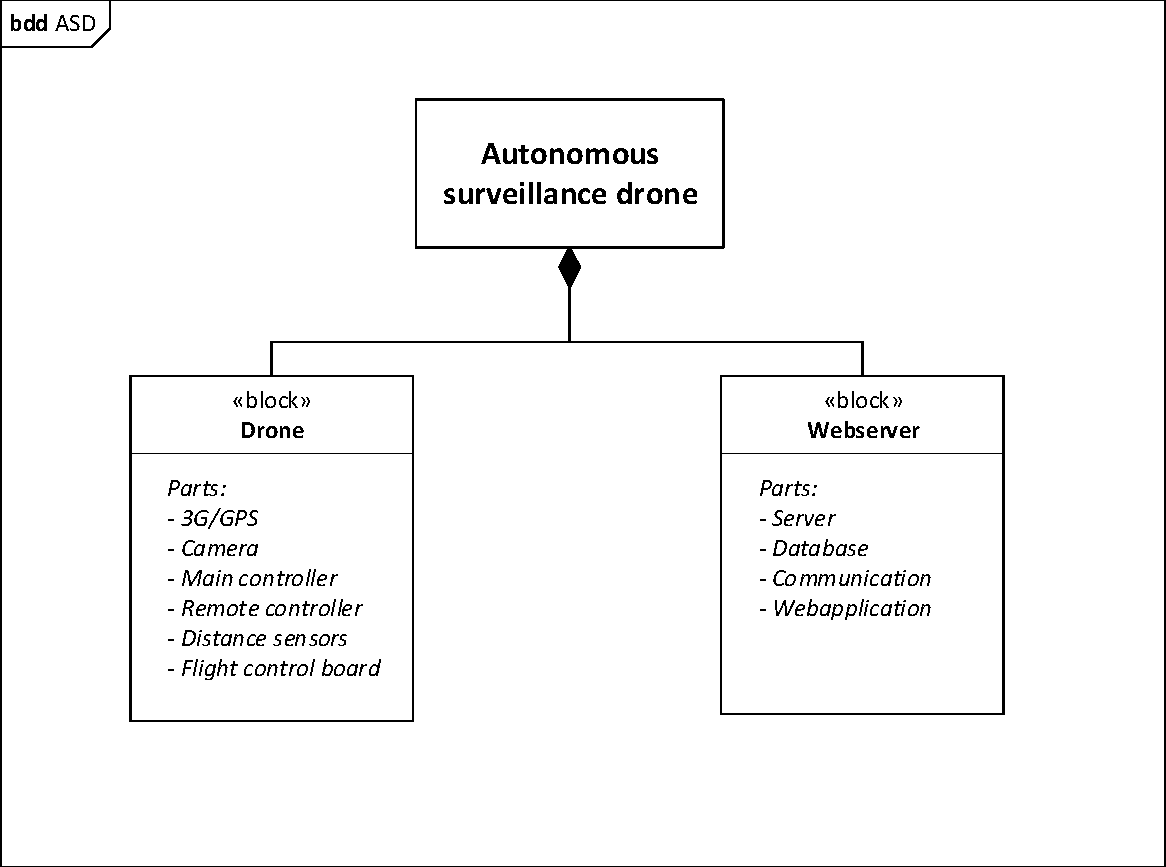
\includegraphics[width=1.0\textwidth]{Billeder/Projektbeskrivelse/bdd_overordnet.pdf}
	\caption{Overordnet bdd for systemet}
	\label{fig:bdd_asd}
\end{figure}

\textbf{Drone} \\
Drone blokken indeholder alt funktionalitet tilhørende drone. De interne forbindelse mellem de forskellige parts er beskrevet i bdd'er som findes i \textit{Systemarkitektur og Design} [X].

\textbf{Webserver} \\
Webserver blokken indeholder server, database, communication og webapplikationen.

\newpage

\subsection{Interne forbindelser}
\vspace{-0.3cm}	
Det overordnede ibd for systemet vises på figur \ref{fig:ibd_asd}. Dels beskriver ibd'et hvordan  systemets største blokke kommunikerer med hinanden og omverden. Desuden beskriver ibd'et hvilken type signaler der anvendes mellem blokke og omverden. 

\begin{figure}[H]
	\centering
	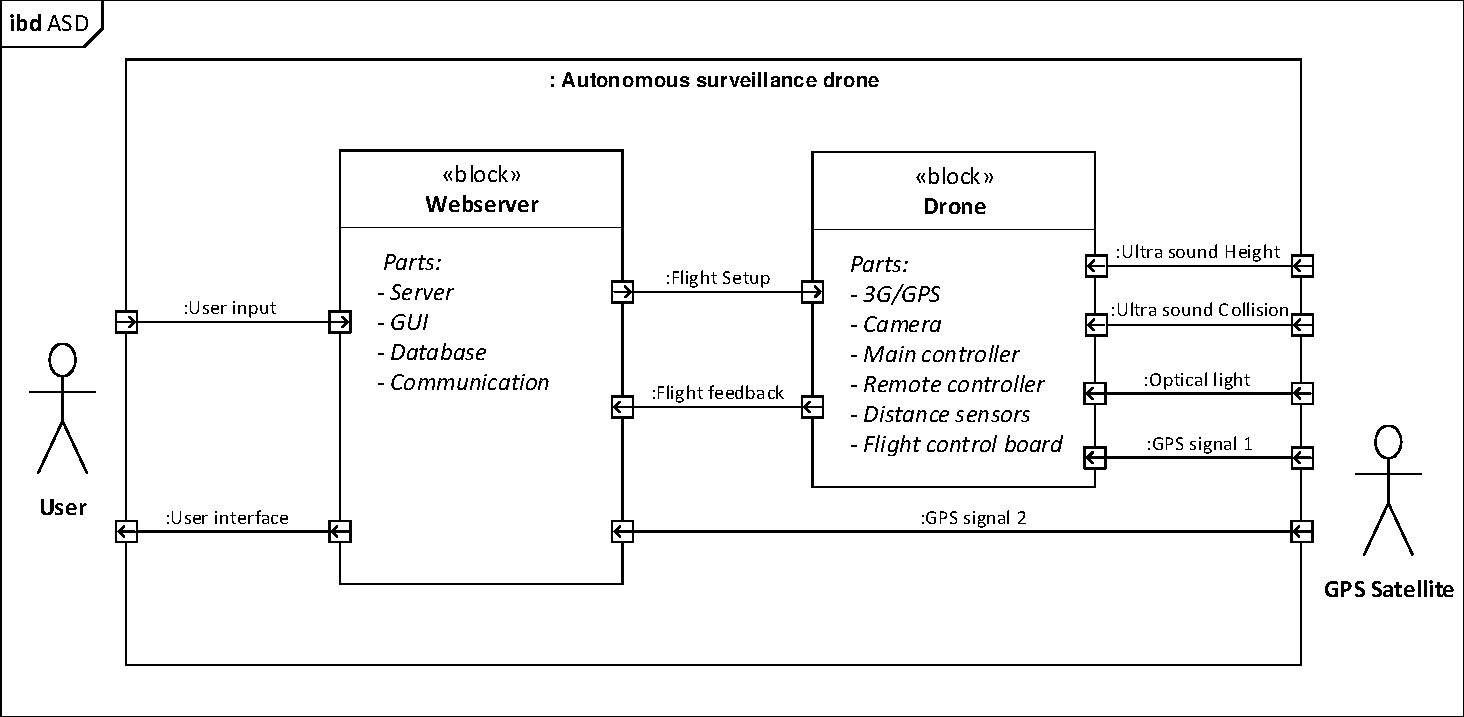
\includegraphics[width=1\textwidth]{Billeder/Projektbeskrivelse/ibd1_overordnet.pdf}
	\caption{Overordnet ibd for systemet}
	\label{fig:ibd_asd}
\end{figure}

Der vises ikke udvidede ibd'er for webserver, da webserver beskrives med UML i stedet for SysML. 
For en beskrivelse af alle udarbejdede ibd'er til drone henvises til dokumentationens \textit{Systemarkitektur og Design} [X].

\subsection{Pakke diagram}
\vspace{-0.3cm}	
Pakkediagrammer bruges i software design afsnittet til at vise hvilke ansvarsområder hver pakke har. På figur \ref{fig:package_drone} ses de overordnede pakker tilhørende dronen. Pakkerne og deres ansvarsområde bruges til at danne grundlag for udformning af softwareklasser og klassernes indbyrdes forhold.
 
\begin{figure}[H]
	\centering
	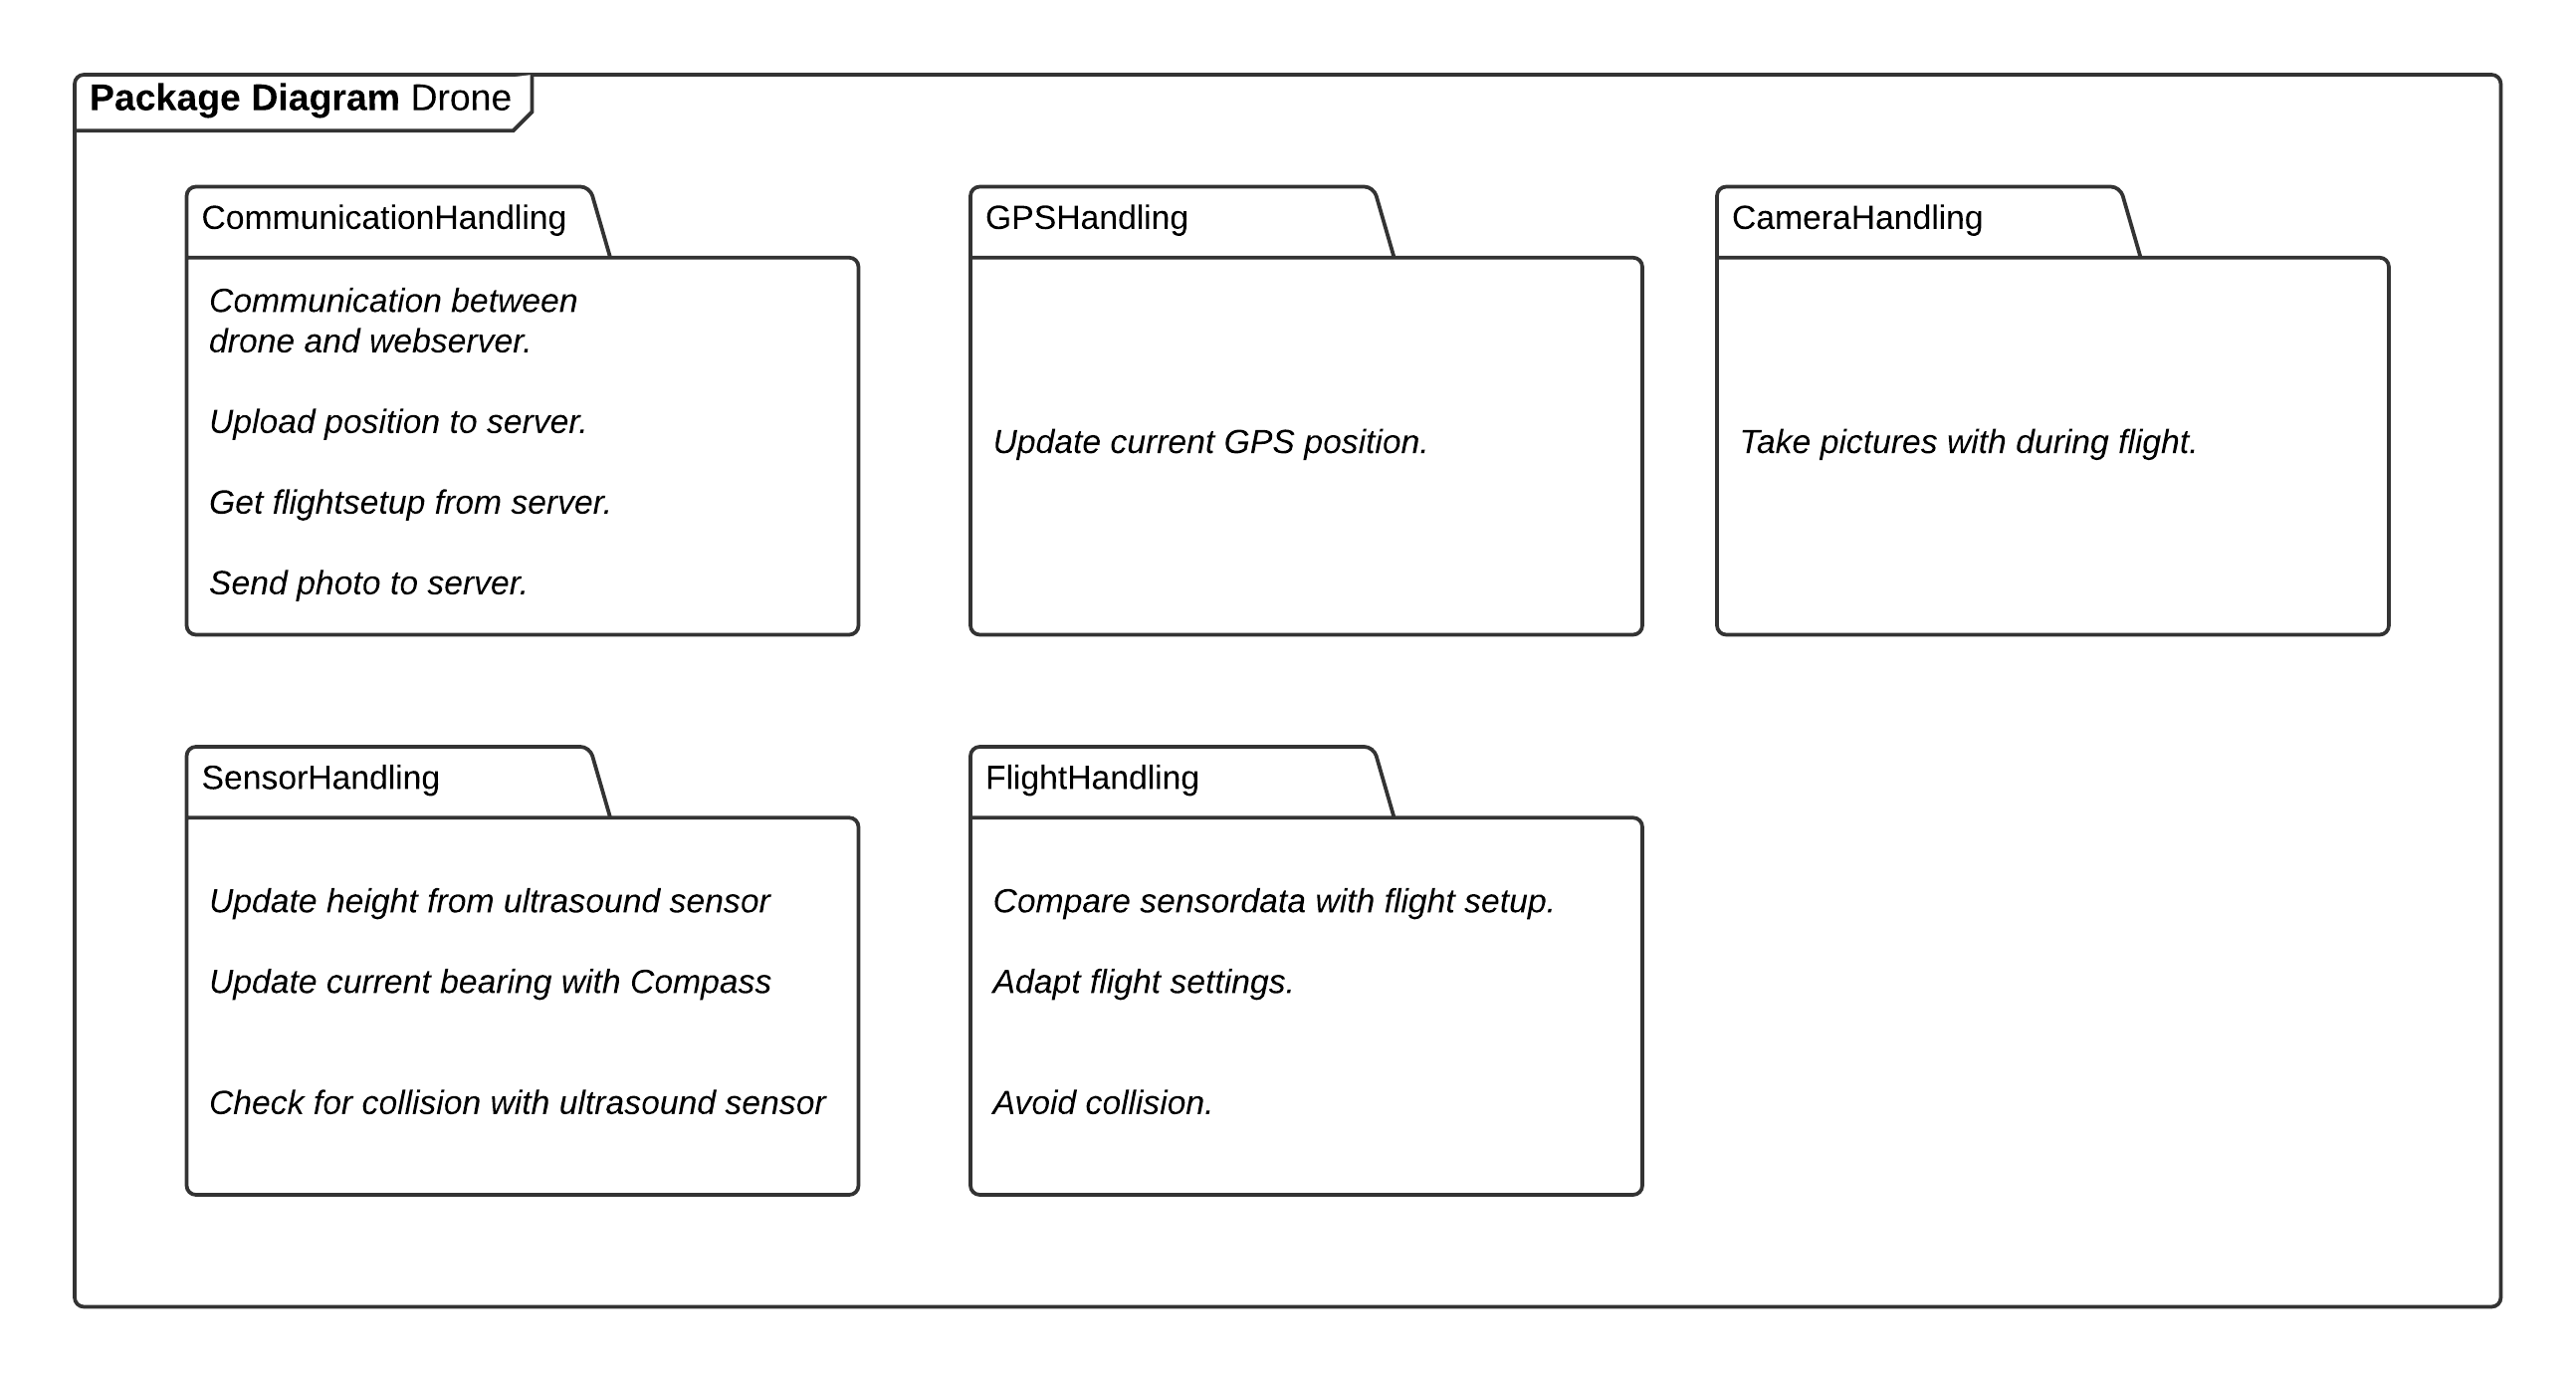
\includegraphics[width=0.85\textwidth]{Billeder/Projektbeskrivelse/Packagediagram_drone}
	\vspace{-0.3cm}	
	\caption{Overordnet pakkediagram for drone}
	\label{fig:package_drone}
\end{figure}